\documentclass{article}
\usepackage[margin = 0.5in]{geometry}
\usepackage{amsfonts, setspace, graphicx}
\graphicspath{{./images/}}
\begin{document}
    \onehalfspacing

    \begin{singlespace}
        \title{CSE 417T: Homework 1} 
        \author{Hangxiao Zhu}
        \date{\today}
        \maketitle
    \end{singlespace}

    \section*{Problem 1.}
    I'm going to show the proof in the following steps.\\
    (a) Since $\mathbf{w^*}$ is an optimal set of weights, $\mathbf{w^*}^T \mathbf{x}_n$ must yields the same
    sign as $y_n$. That is, $sign(\mathbf{w^*}^T \mathbf{x}_n) = y_n$. Therefore, we can deduce that 
    $y_n(\mathbf{w^*}^T \mathbf{x}_n) > 0$ for any $n \in [1, N]$. Therefore, when 
    $\rho = min_{1 \leq n \leq N}y_n(\mathbf{w^*}^T \mathbf{x}_n)$, it is guaranteed that $\rho > 0$.\\
    (b) We will prove by induction:\\
    \textbf{Base case}: When $t = 1$, $\mathbf{w}^T(t-1)\mathbf{w^*} + \rho = 
    \mathbf{w}^T(0)\mathbf{w^*} + \rho = \mathbf{0}\mathbf{w^*} + \rho = \rho$, and 
    $\mathbf{w}^T(t) \mathbf{w^*} = \mathbf{w}^T(1)\mathbf{w^*}$.\\
    By Perceptron Learning Algorithm, we know 
    $\mathbf{w}^T(t+1) = \mathbf{w}^T(t) + y_n\mathbf{x}_n^T$ for some $n \in [1, N]$.
    Therefore, by choosing a random $n \in [1, N]$, $\mathbf{w}^T(1) = \mathbf{w}^T(0) + y_n\mathbf{x}_n^T = 
    \mathbf{0} + y_n\mathbf{x}_n^T = y_n\mathbf{x}_n^T$, which leads to 
    $\mathbf{w}^T(1)\mathbf{w^*} = y_n\mathbf{x}_n^T \mathbf{w^*} = 
    y_n\mathbf{w^*}^T \mathbf{x}_n$.\\
    By definition of $\rho$, we know $y_n\mathbf{w^*}^T \mathbf{x}_n \geq \rho$, therefore, 
    $\mathbf{w}^T(1)\mathbf{w^*} \geq \rho$.
    Since $\mathbf{w}^T(0)\mathbf{w^*} + \rho = \rho$,
    $\mathbf{w}^T(1) \mathbf{w^*} = \mathbf{w}^T(1)\mathbf{w^*}$, and $\mathbf{w}^T(1)\mathbf{w^*} \geq \rho$,
    we can deduce that $\mathbf{w}^T(t)\mathbf{w^*} \geq \mathbf{w}^T(t-1)\mathbf{w^*} + \rho$ is true for 
    $t = 1$.\\
    \textbf{Induction Step}: Assume $\mathbf{w}^T(t)\mathbf{w^*} \geq \mathbf{w}^T(t-1)\mathbf{w^*} + \rho$ is 
    true for $t \in \mathbb{N}$. We need to prove 
    $\mathbf{w}^T(t+1)\mathbf{w^*} \geq \mathbf{w}^T(t)\mathbf{w^*} + \rho$ is still true.\\
    By Perceptron Learning Algorithm, we know $\mathbf{w}^T(t+1) = \mathbf{w}^T(t) + y_n\mathbf{x}_n^T$ for 
    some $n \in [1, N]$. Therefore, by choosing a random $n \in [1, N]$, 
    $\mathbf{w}^T(t+1)\mathbf{w^*} = \mathbf{w}^T(t) \mathbf{w^*} + y_n\mathbf{x}_n^T \mathbf{w^*} \geq
    \mathbf{w}^T(t-1) \mathbf{w^*} + \rho +  y_n\mathbf{x}_n^T \mathbf{w^*} \geq
    [\mathbf{w}^T(t-1) + y_n\mathbf{x}_n^T] \mathbf{w^*} + \rho \geq
    \mathbf{w}^T(t)\mathbf{w^*} + \rho$.\\
    Thus, $\mathbf{w}^T(t+1)\mathbf{w^*} \geq \mathbf{w}^T(t)\mathbf{w^*} + \rho$ still holds, and the proof of 
    the induction step is complete.\\
    \textbf{Conclusion}: By the principle of induciton, 
    $\mathbf{w}^T(t)\mathbf{w^*} \geq \mathbf{w}^T(t-1)\mathbf{w^*} + \rho$ is true for all $t \in \mathbb{N}$.
    Then, we can easily deduce that $\mathbf{w}^T(t)\mathbf{w^*} \geq \mathbf{w}^T(t-1)\mathbf{w^*} + \rho \geq
    \mathbf{w}^T(t-2)\mathbf{w^*} + 2\rho \geq \mathbf{w}^T(t-3)\mathbf{w^*} + 3\rho \geq \cdots \geq 
    \mathbf{w}^T(0)\mathbf{w^*} + t\rho = t\rho$.\\
    (c) By Perceptron Learning Algorithm, we know $\mathbf{w}(t) = \mathbf{w}(t-1) + y(t-1)\mathbf{x}(t-1)$. 
    Therefore, $||\mathbf{w}(t)||^2 = ||\mathbf{w}(t-1)||^2 + ||y(t-1)\mathbf{x}(t-1)||^2 + 
    2\mathbf{w}^T(t-1)y(t-1)\mathbf{x}(t-1) = 
    ||\mathbf{w}(t-1)||^2 + y(t-1)^2||\mathbf{x}(t-1)||^2 + 2y(t-1)\mathbf{w}^T(t-1)\mathbf{x}(t-1)$.\\
    Since $y$ is either $1$ or $-1$, we know that $y(t-1)^2 = 1$. Besides, since $\mathbf{x}(t-1)$ was 
    misclassified, we know that $y(t-1)*(\mathbf{w}^T(t-1)\mathbf{x}(t-1)) \leq 0$.\\
    By substituting these results into the above equation, we have $||\mathbf{w}(t)||^2 = 
    ||\mathbf{w}(t-1)||^2 + ||\mathbf{x}(t-1)||^2 + 2y(t-1)\mathbf{w}^T(t-1)\mathbf{x}(t-1) \leq
    ||\mathbf{w}(t-1)||^2 + ||\mathbf{x}(t-1)||^2$.\\
    (d) We will prove by induction:\\
    \textbf{Base case}: When $t = 0$, $\mathbf{w}(0) = \mathbf{0}, tR^2 = 0$. Therefore, 
    $||\mathbf{w}(0)||^2 = 0$. We can deduce that $||\mathbf{w}(t)||^2 \leq tR^2$ is true for $t = 0$.\\
    \textbf{Induction Step}: Assume $||\mathbf{w}(t-1)||^2 \leq (t-1)R^2$ is true for $(t-1) \in \mathbb{N}$. We 
    need to prove $||\mathbf{w}(t)||^2 \leq tR^2$ is still true.\\
    Based on the conclusion from (c), $||\mathbf{w}(t)||^2 \leq ||\mathbf{w}(t-1)||^2 + ||\mathbf{x}(t-1)||^2$.
    Since $R = max_{1 \leq n \leq N}||\mathbf{x}_n||$, we know that $||\mathbf{w}(t)||^2 \leq (t-1)R^2 + R^2 =
    tR^2$.\\
    Thus, $||\mathbf{w}(t)||^2 \leq tR^2$ still holds, and the proof of the induction step is complete.\\
    \textbf{Conclusion}: By the principle of induciton, $||\mathbf{w}(t)||^2 \leq tR^2$ is true for all 
    $t \in \mathbb{N}$.\\
    (e) Based on the conclusion from (b), $\frac{\mathbf{w}^T(t)\mathbf{w^*}}{||\mathbf{w}(t)||} \geq 
    \frac{t\rho}{||\mathbf{w}(t)||}$. Based on the conclusion from (d), $||\mathbf{w}(t)|| \leq \sqrt{t}R$.\\
    By substituting the second inequality into the first inequality, we can deduce that 
    $\frac{\mathbf{w}^T(t)\mathbf{w^*}}{||\mathbf{w}(t)||} \geq \frac{t\rho}{||\mathbf{w}(t)||} \geq 
    \frac{t\rho}{\sqrt{t}R} = \sqrt{t}\frac{\rho}{R}$.\\
    Based on the inequality above, $\sqrt{t} \leq 
    \frac{\mathbf{w}^T(t)\mathbf{w^*}}{||\mathbf{w}(t)||} \cdot \frac{R}{\rho}$. Therefore, $t \leq
    \frac{(\mathbf{w}^T(t)\mathbf{w^*})^2}{||\mathbf{w}(t)||^2} \cdot \frac{R^2}{\rho^2} = 
    \frac{R^2||\mathbf{w^*}||^2}{\rho^2}$.\\
    Based on the conclusion fron (e), we know that Perceptron Learning Algorithm will give the solution after 
    $t$ iterations, where $t \leq \frac{R^2||\mathbf{w^*}||^2}{\rho^2}$ and 
    $\frac{R^2||\mathbf{w^*}||^2}{\rho^2} \in \mathbb{N}$. This means Perceptron Learning Algorithm
    eventually converges. Q.E.D
    
    \section*{Problem 2.}
    I attached two graphs below. Figure 1 is the Histogram of Number of Iterations. Figure 2 is the Histogram of 
    Log Difference of Theoretical Bounds and Actual Number of Iterations.
        \begin{figure}[!htb]
            \begin{center}
                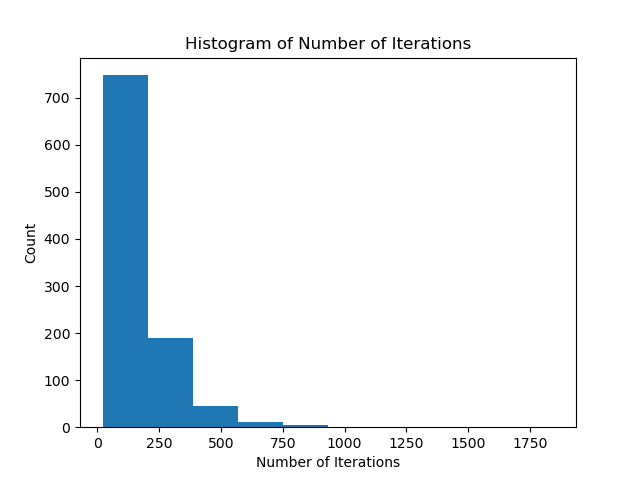
\includegraphics[width=10cm, height=8cm]{NumberOfIterations}
                \textbf{\caption{Histogram of Number of Iterations}}
                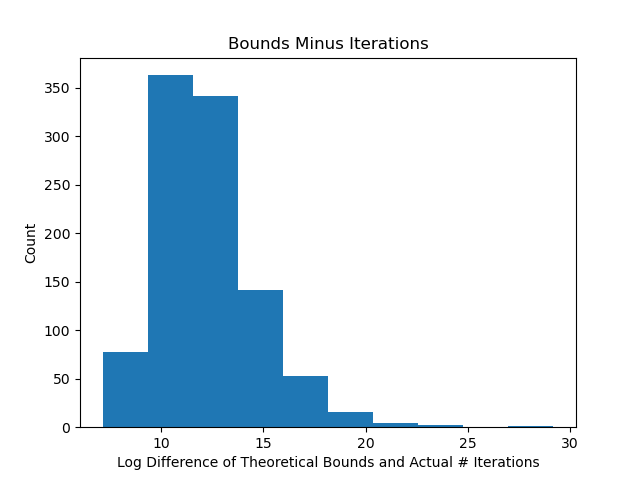
\includegraphics[width=10cm, height=8cm]{BoundsMinusIterations}
                \textbf{\caption{Histogram of Log Difference of Theoretical Bounds and Actual Number of Iterations}}
            \end{center}
        \end{figure}\\
    \textbf{Interpretations of the results}: According to the first graph, we know that the number of cycles 
    required for most experiments is less than 500. In particular, most of them are concentrated around 200. This 
    implies that when the size of the data set is fixed, Perceptron Learning Algorithm can always converge 
    within a certain number of iterations most of the time.\\ 
    According to the second graph, we know that the log difference of theoretical bounds and actual number of 
    iterations is less than 20. In particular, most of them are concentrated around 12. This implies that the 
    theoretical boundary is a very loose limit, and in most cases, Perceptron Learning Algorithm is able to converge 
    at a much smaller number of iterations than the theoretical bound.

    \section*{Problem 3.}
    (a) The value of $\mu$ for each of the three selected coins is 0.5, because they are all fair coins.\\
    (b) I attached three histograms of the distributions of $v_1$, $v_rand$, and $v_min$.
    \begin{figure}[!htb]
        \begin{center}
            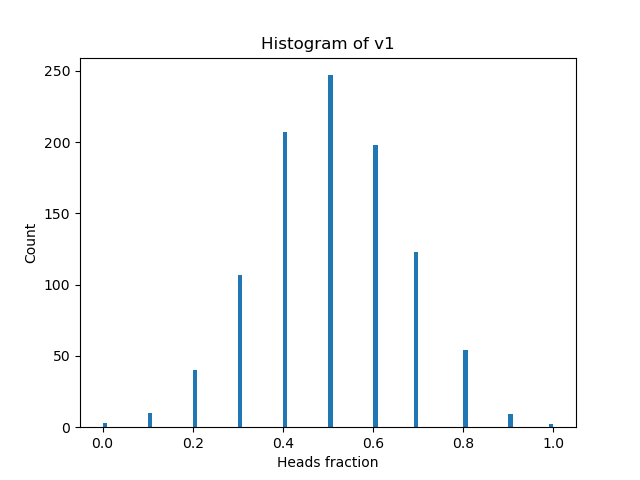
\includegraphics[width=8cm, height=6cm]{v1}
            \textbf{\caption{Histogram of $v_1$}}
            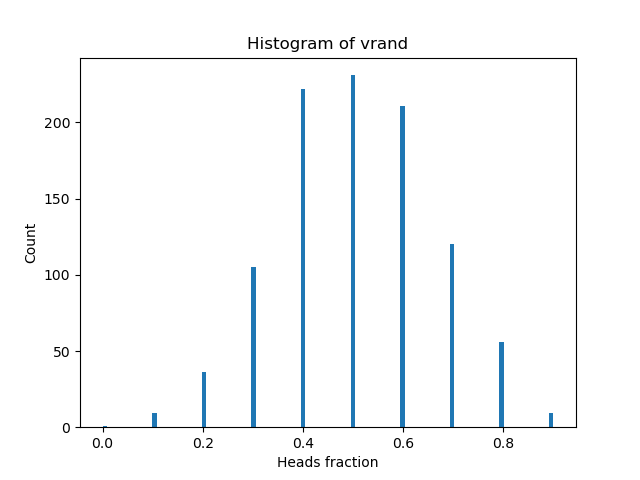
\includegraphics[width=8cm, height=6cm]{vrand}
            \textbf{\caption{Histogram of $v_rand$}}
            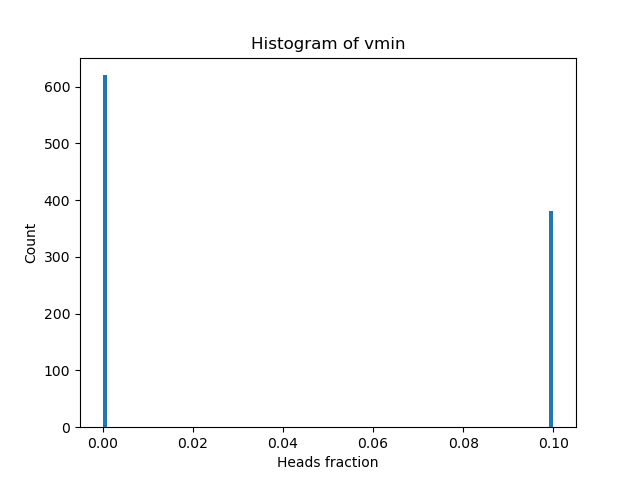
\includegraphics[width=8cm, height=6cm]{vmin}
            \textbf{\caption{Histogram of $v_min$}}
        \end{center}
    \end{figure}\\
    (c) I attached the grapgh showing estimates for $\mathbb{P}[|v-\mu|>\epsilon]$ as a function of $\epsilon$,
    together with the Hoeffding bound.
    \begin{figure}[!htb]
        \begin{center}
            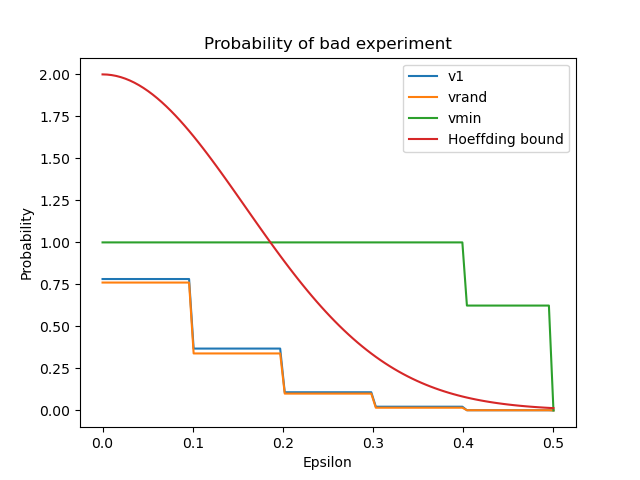
\includegraphics[width=8cm, height=6cm]{bad}
            \textbf{\caption{Estimates for $\mathbb{P}[|v-\mu|>\epsilon]$}}
        \end{center}
    \end{figure}\\
    \\
    \\
    (d) The first coin and the random coin obey the Hoeffding bound, while the minimum-frequency-of-heads coin
    doesn't obey the Hoeffding bound. Beacuse the Hoeffding bound can only be adapted when the hypothesis $h$ 
    be "fixed" before the experiment. In this scenario, it means "choosing the coins before sampleing". It's
    apparently that only the first coin and the random coin were drawn under this restriction.\\
    (e) Our operation of selecting coins can be analogous to selecting one bin from 1000 bins. The first two bins 
    are selected before sampling, and the last bin is selected after completing data sampling. Thus only the first 
    two bins can depict this learning problem, and the last selected bin is not justified.

    \section*{Problem 4.}
    (a) According to the law of total expectation, $\mathbb{E}(t) = \mathbb{E}(t|t<\alpha) \mathbb{P}(t<\alpha) +
    \mathbb{E}(t|t \geq \alpha) \mathbb{P}(t \geq \alpha)$. Therefore $\frac{\mathbb{E}(t)}{\alpha} = 
    \frac{\mathbb{E}(t|t<\alpha) \mathbb{P}(t<\alpha)}{\alpha} + 
    \frac{\mathbb{E}(t|t \geq \alpha) \mathbb{P}(t \geq \alpha)}{\alpha}$.\\
    Since $t$ is a non negative random variable, we can deduce that 
    $\frac{\mathbb{E}(t|t \geq \alpha)}{\alpha} \geq 1$. Therefore $\frac{\mathbb{E}(t)}{\alpha} \geq 
    \frac{\mathbb{E}(t|t<\alpha) \mathbb{P}(t<\alpha)}{\alpha} + \mathbb{P}(t \geq \alpha)$.\\
    Since $\alpha > 0$ and $t$ is a non negative random variable, we can deduce that 
    $\frac{\mathbb{E}(t|t<\alpha) \mathbb{P}(t<\alpha)}{\alpha} > 0$. Therefore $\frac{\mathbb{E}(t)}{\alpha} \geq 
    \mathbb{P}(t \geq \alpha)$, which is $\mathbb{P}(t \geq \alpha) \leq \frac{\mathbb{E}(t)}{\alpha}$.\\
    (b) Since $(u - \mu)^2 \geq 0$, and $\sigma^2 = \mathbb{E}((u - \mu)^2)$, based on the conclusion from (a), we 
    can deduce that $\mathbb{P}[(u - \mu)^2 \geq \alpha] \leq \frac{\sigma^2}{\alpha}$.
    (c) Since $u = \frac{1}{N}\sum_{n=1}^N u_n$, we can calculate $u$ has mean $\mu$ and variance 
    $\frac{\sigma^2}{N}$. Based on the conclusion from (b), we can deduce that $\mathbb{P}[(u - \mu)^2 \geq \alpha] 
    \leq \frac{\frac{\sigma^2}{N}}{\alpha} = \frac{\sigma^2}{N \alpha}$.

    \section*{Problem 5.}
    (a) To minimize $E_{in}(h) = \sum_{n=1}^{N}(h - y_n)^2$, we need to take deriviate of $E_{in}(h)$ and find the 
    extrema point. Therefore, we do $\frac{\partial E_{in}(h)}{\partial h} = 2\sum_{n=1}^{N}(h - y_n) = 0$. By soving 
    this equation, we get $h = \frac{1}{N}\sum_{n=1}^{N}y_n$. And we know $h_{mean} = \frac{1}{N}\sum_{n=1}^{N}y_n$. 
    Thus, we know $h$ is in sample mean $h_{mean}$.\\
    (b) To minimize $E_{in}(h) = \sum_{n=1}^{N}|h - y_n|$, we need to take deriviate of $E_{in}(h)$ and find the 
    extrema point. Therefore, we do $\frac{\partial E_{in}(h)}{\partial h} = \sum_{n=1}^{N}sign(h - y_n) = 0$. To 
    ensure that this equation has a solution, we need to ensure half of the data points are at most $h$ and half of 
    the data points are at least $h$. And we know half of the data points are at most $h_{med}$ and half of the data 
    points are at least $h_{med}$. Thus, we know $h$ is in sample median $h_{med}$.\\
    (c) With $y_N$ be pertuebed to $y_N + \epsilon$, and $\epsilon \to \infty$, we know $y_N \to \infty$. Therefore, 
    $\sum_{n=1}^{N}y_n \to \infty$, which leads to $h_{mean} \to \infty$. However, before $y_N$ be pertuebed, 
    $y_1 \leq \cdots \leq y_N$, we know $h_{med} < y_N$. And after $y_N$ be pertuebed, $h_{med} < y_N$ is still true.
    Therefore, $h_{med}$ stay the same.

    \section*{Problem 6.}
    (a) When $\mathcal{H} = Positive\:Rays$, $m_{\mathcal{H}}(N) = N + 1$. When $\mathcal{H} = Negative\:Rays$, 
    $m_{\mathcal{H}}(N) = N + 1$. And these two scenarios have two overlapped situation, when 
    $\mathcal{H}(\mathbf{x_1}, \mathbf{x_2}, \cdots, \mathbf{x_N}) = \{+1, +1, \cdots, +1\}$ and 
    $\mathcal{H}(\mathbf{x_1}, \mathbf{x_2}, \cdots, \mathbf{x_N}) = \{-1, -1, \cdots, -1\}$. Therefore when 
    $\mathcal{H} = Positive\:or\:Negative\:Rays$, $m_{\mathcal{H}}(N) = 2N$.\\
    Since the smallest break point $N$ which satisfies $m_{\mathcal{H}}(N) > 2^N$ is $3$, the VC dimenstion 
    $d_{VC}(H) = 2$.\\
    (b) When $\mathcal{H} = Positive\:Intervals$, $m_{\mathcal{H}}(N) = C_2^{N+1} + 1 = \frac{N^2 + N}{2} + 1$. 
    When $\mathcal{H} = Negative\:Intervals$, though $m_{\mathcal{H}}(N) = C_2^{N+1} + 1 = \frac{N^2 + N}{2} + 1$,
    the new $\mathcal{H}$ we get is $N - 2$. Therefore when $\mathcal{H} = Positive\:or\:Negative\:Intervals$,
    $m_{\mathcal{H}}(N) = \frac{N^2 + 3N}{2} - 1$.\\ 
    Since the smallest break point $N$ which satisfies $m_{\mathcal{H}}(N) > \frac{N^2 + 3N}{2} - 1$ is $4$, the VC 
    dimenstion $d_{VC}(H) = 3$.\\
    (c) This learning model should have the same $m_{\mathcal{H}}(N)$ as $\mathcal{H} = Positive\:Intervals$,
    therefore $m_{\mathcal{H}}(N) = C_2^{N+1} + 1 = \frac{N^2 + N}{2} + 1$, the VC dimenstion $d_{VC}(H) = 2$.
\end{document}